% =============================================================================
% Intro của section "Thiết kế chi tiết các thành phần"
% Đặt ngay sau \section{Thiết kế chi tiết các thành phần} và trước các \input{}
% =============================================================================

\section{Thiết kế chi tiết các thành phần}
\label{sec:detailed-components}

Mục 3.2 đã trình bày kiến trúc tổng quan và đặt mỗi thành phần vào một vị trí trên sơ đồ off-chain/on-chain; mục \S\ref{sec:three-layer-model} bổ sung góc nhìn \emph{chiến lược thực thi} bằng mô hình ba lớp Netting $\rightarrow$ Accelerator $\rightarrow$ Fallback. Hai mục đó trả lời các câu hỏi ``hệ thống có những gì'' và ``một intent đi qua đâu trước, đâu sau''.

Mục này đào sâu vào từng thành phần riêng lẻ. Với mỗi thành phần, khoá luận trình bày trách nhiệm, cấu trúc dữ liệu, các thuật toán cốt lõi, quan hệ tương tác với các thành phần khác và những đánh đổi thiết kế cụ thể đã được lựa chọn. Việc tách rời mỗi thành phần thành một mục con riêng cho phép người đọc tham khảo nhanh từng module mà không phải đọc tuần tự cả chương, đồng thời tránh trùng lặp với các phần dẫn nhập ở trên.

Bảy thành phần được trình bày theo thứ tự đi từ ngoài vào trong, bám sát luồng xử lý của một intent điển hình. Đầu tiên là Smart Contract Layer (HTLC), tầng on-chain và là điểm cuối nơi tài sản thực sự bị khoá và giải phóng; mục này mô tả HTLC chuẩn, biến thể \emph{multi-fill} của OceanLink, và cách hashlock được chia sẻ giữa các nhánh để đảm bảo tính nguyên tử của một chu trình. Tiếp đến là API Gateway, cổng vào duy nhất của backend, với bốn nhóm route, hàm \texttt{validateIntent}, kênh Server-Sent Events, và cách module Risk engine trong sơ đồ ý đồ được hợp nhất vào tầng này ở quy mô MVP.

Order Book (OrderStore) là sổ lệnh in-memory với cơ chế write-through xuống Postgres. Mục này làm rõ sự phân tách giữa ``nguồn sự thật lúc chạy'' (in-memory) và ``lưu trữ bền'' (database), cũng như quá trình \texttt{hydrate()} khi tiến trình khởi động. Matching Engine là hạt nhân của lớp Netting; mục này mô hình hoá orderbook thành đồ thị có hướng, mô tả vòng lặp điều phối tick, và đặc biệt là \emph{thuật toán giảm chu trình (cycle-reduction)} với pseudocode, ví dụ minh hoạ và phân tích độ phức tạp.

Execution Engine, gồm Orchestrator và BridgeService, là tầng biến \texttt{MatchResult} thành các giao dịch on-chain. Mục này trình bày mô hình \emph{presiding/responding orders}, thuật toán \texttt{handleMatchResults} chín bước, và phân tích bốn tình huống lỗi để chứng minh tính nguyên tử được duy trì trong mọi trường hợp. Fallback Bridge Aggregator (chỉ ở mức thiết kế ý đồ) là lớp cuối cùng, định tuyến qua bridge bên thứ ba khi hai lớp trên không xử lý được intent; mục này trình bày interface \texttt{BridgeAdapter} và các bridge ứng cử (Across, LayerZero, Chainlink CCIP), còn cài đặt cụ thể được liệt kê ở Future Work. Cuối cùng, Event Bus và Persistence trình bày hai cơ chế tách biệt cùng đóng vai trò \emph{event log}: Postgres cho durable state và \texttt{EventEmitter} trong bộ nhớ cho transient pub/sub. Mục này làm rõ tại sao thiết kế này là sự thay thế hợp lý cho một Kafka topic ở quy mô MVP.

Trong mỗi mục con, các trường hợp lỗi và các đánh đổi thiết kế được nêu rõ. Phân tích đánh giá tổng thể (so sánh thuật toán, đo benchmark, so sánh với các bridge khác) được dành cho chương Đánh giá.

% -----------------------------------------------------------------------------
% Includes — uncomment phần \input dưới đây sau khi đã review từng file con.
% -----------------------------------------------------------------------------

% =============================================================================
% Draft mục 3.3.1 — Smart Contract Layer (HTLC)
% Đặt trong c3/ và \input{} vào c3_chapter.tex sau khi rà soát.
% =============================================================================

\subsection{Smart Contract Layer (HTLC)}
\label{sec:smart-contract-layer}

Lớp smart contract là tầng cao nhất quyết định việc chuyển giao tài sản
giữa các chuỗi. Trong OceanLink, lớp này gồm ba phiên bản giống nhau của
hợp đồng \texttt{HashedTimelockERC20} được triển khai trên Ethereum, Arbitrum và Base. Hợp đồng cài đặt một biến
thể \emph{multi-fill} của giao thức Hashed Time-Locked Contract (HTLC)
nhằm hỗ trợ thanh toán nguyên tử (atomic settlement) cho cả các vòng
khớp lệnh nhiều bên do Matching Engine tạo ra.

\subsubsection*{Thuật toán HTLC}

HTLC là một thuật toán mật mã đã được phát triển từ lâu nhưng chưa được thương mại
hoá rộng rãi, nó được biết đến chủ yếu trong giới nghiên cứu và một
số giao thức thanh toán xuyên chuỗi điển hình như Lightning Network
và các giao thức atomic swap giữa Bitcoin và Ethereum, song vẫn chưa
hiện diện trong các sản phẩm bridge thương mại phổ biến hiện nay.
Mô hình cơ bản giữa hai bên $A$ và $B$ trên hai chuỗi khác nhau như
sau:

\begin{enumerate}
  \item Người gửi $A$ chọn một bí mật ngẫu nhiên $s$ và tính
    $h = \mathcal{H}(s)$, với $\mathcal{H}$ là hàm băm an toàn.
  \item \emph{Pha 1 — khởi tạo HTLC trên chuỗi nguồn.} $A$ gọi hợp
    đồng trên chuỗi 1, khoá tài sản với hashlock $h$ và timelock
    $T_A$; thông tin giao dịch được chuyển sang $B$ qua kênh
    off-chain.
  \item \emph{Pha 2 — khởi tạo HTLC đối ứng trên chuỗi đích.} Sau
    khi quan sát được HTLC bên chuỗi 1, $B$ tạo một HTLC tương ứng
    trên chuỗi 2 với cùng hashlock $h$ và timelock $T_B < T_A$ (để
    $B$ luôn còn đủ thời gian xử lý nếu $A$ rút trễ).
  \item \emph{Pha 3 — $A$ rút tài sản trên chuỗi đích.} $A$ cung cấp
    preimage $s$ cho hợp đồng trên chuỗi 2 và nhận tài sản; thao tác
    này \emph{tiết lộ $s$ trên chuỗi}.
  \item \emph{Pha 4 — $B$ rút tài sản trên chuỗi nguồn.} Khi $s$ đã
    công khai, $B$ đọc nó từ event của chuỗi 2 và dùng để rút tài sản
    đã bị $A$ khoá ở Pha 1. Nếu một trong hai bên không hoàn tất
    trước timelock tương ứng, hợp đồng cho phép \emph{refund} tự
    động.
\end{enumerate}

Điểm cốt lõi là \emph{cùng một preimage $s$ mở khoá được nhiều HTLC
khác chuỗi}, nhờ đó mọi nhánh thanh toán hoặc cùng diễn ra hoặc cùng
được hoàn lại — tính nguyên tử (atomicity) được duy trì mà không cần
tin cậy bên thứ ba. Hình \ref{fig:htlc-sequence} minh hoạ bốn pha
trên dưới dạng sequence diagram giữa hai người dùng $A$, $B$ và hai
hợp đồng smart contract trên hai chuỗi.

\begin{figure}[H]
  \centering
  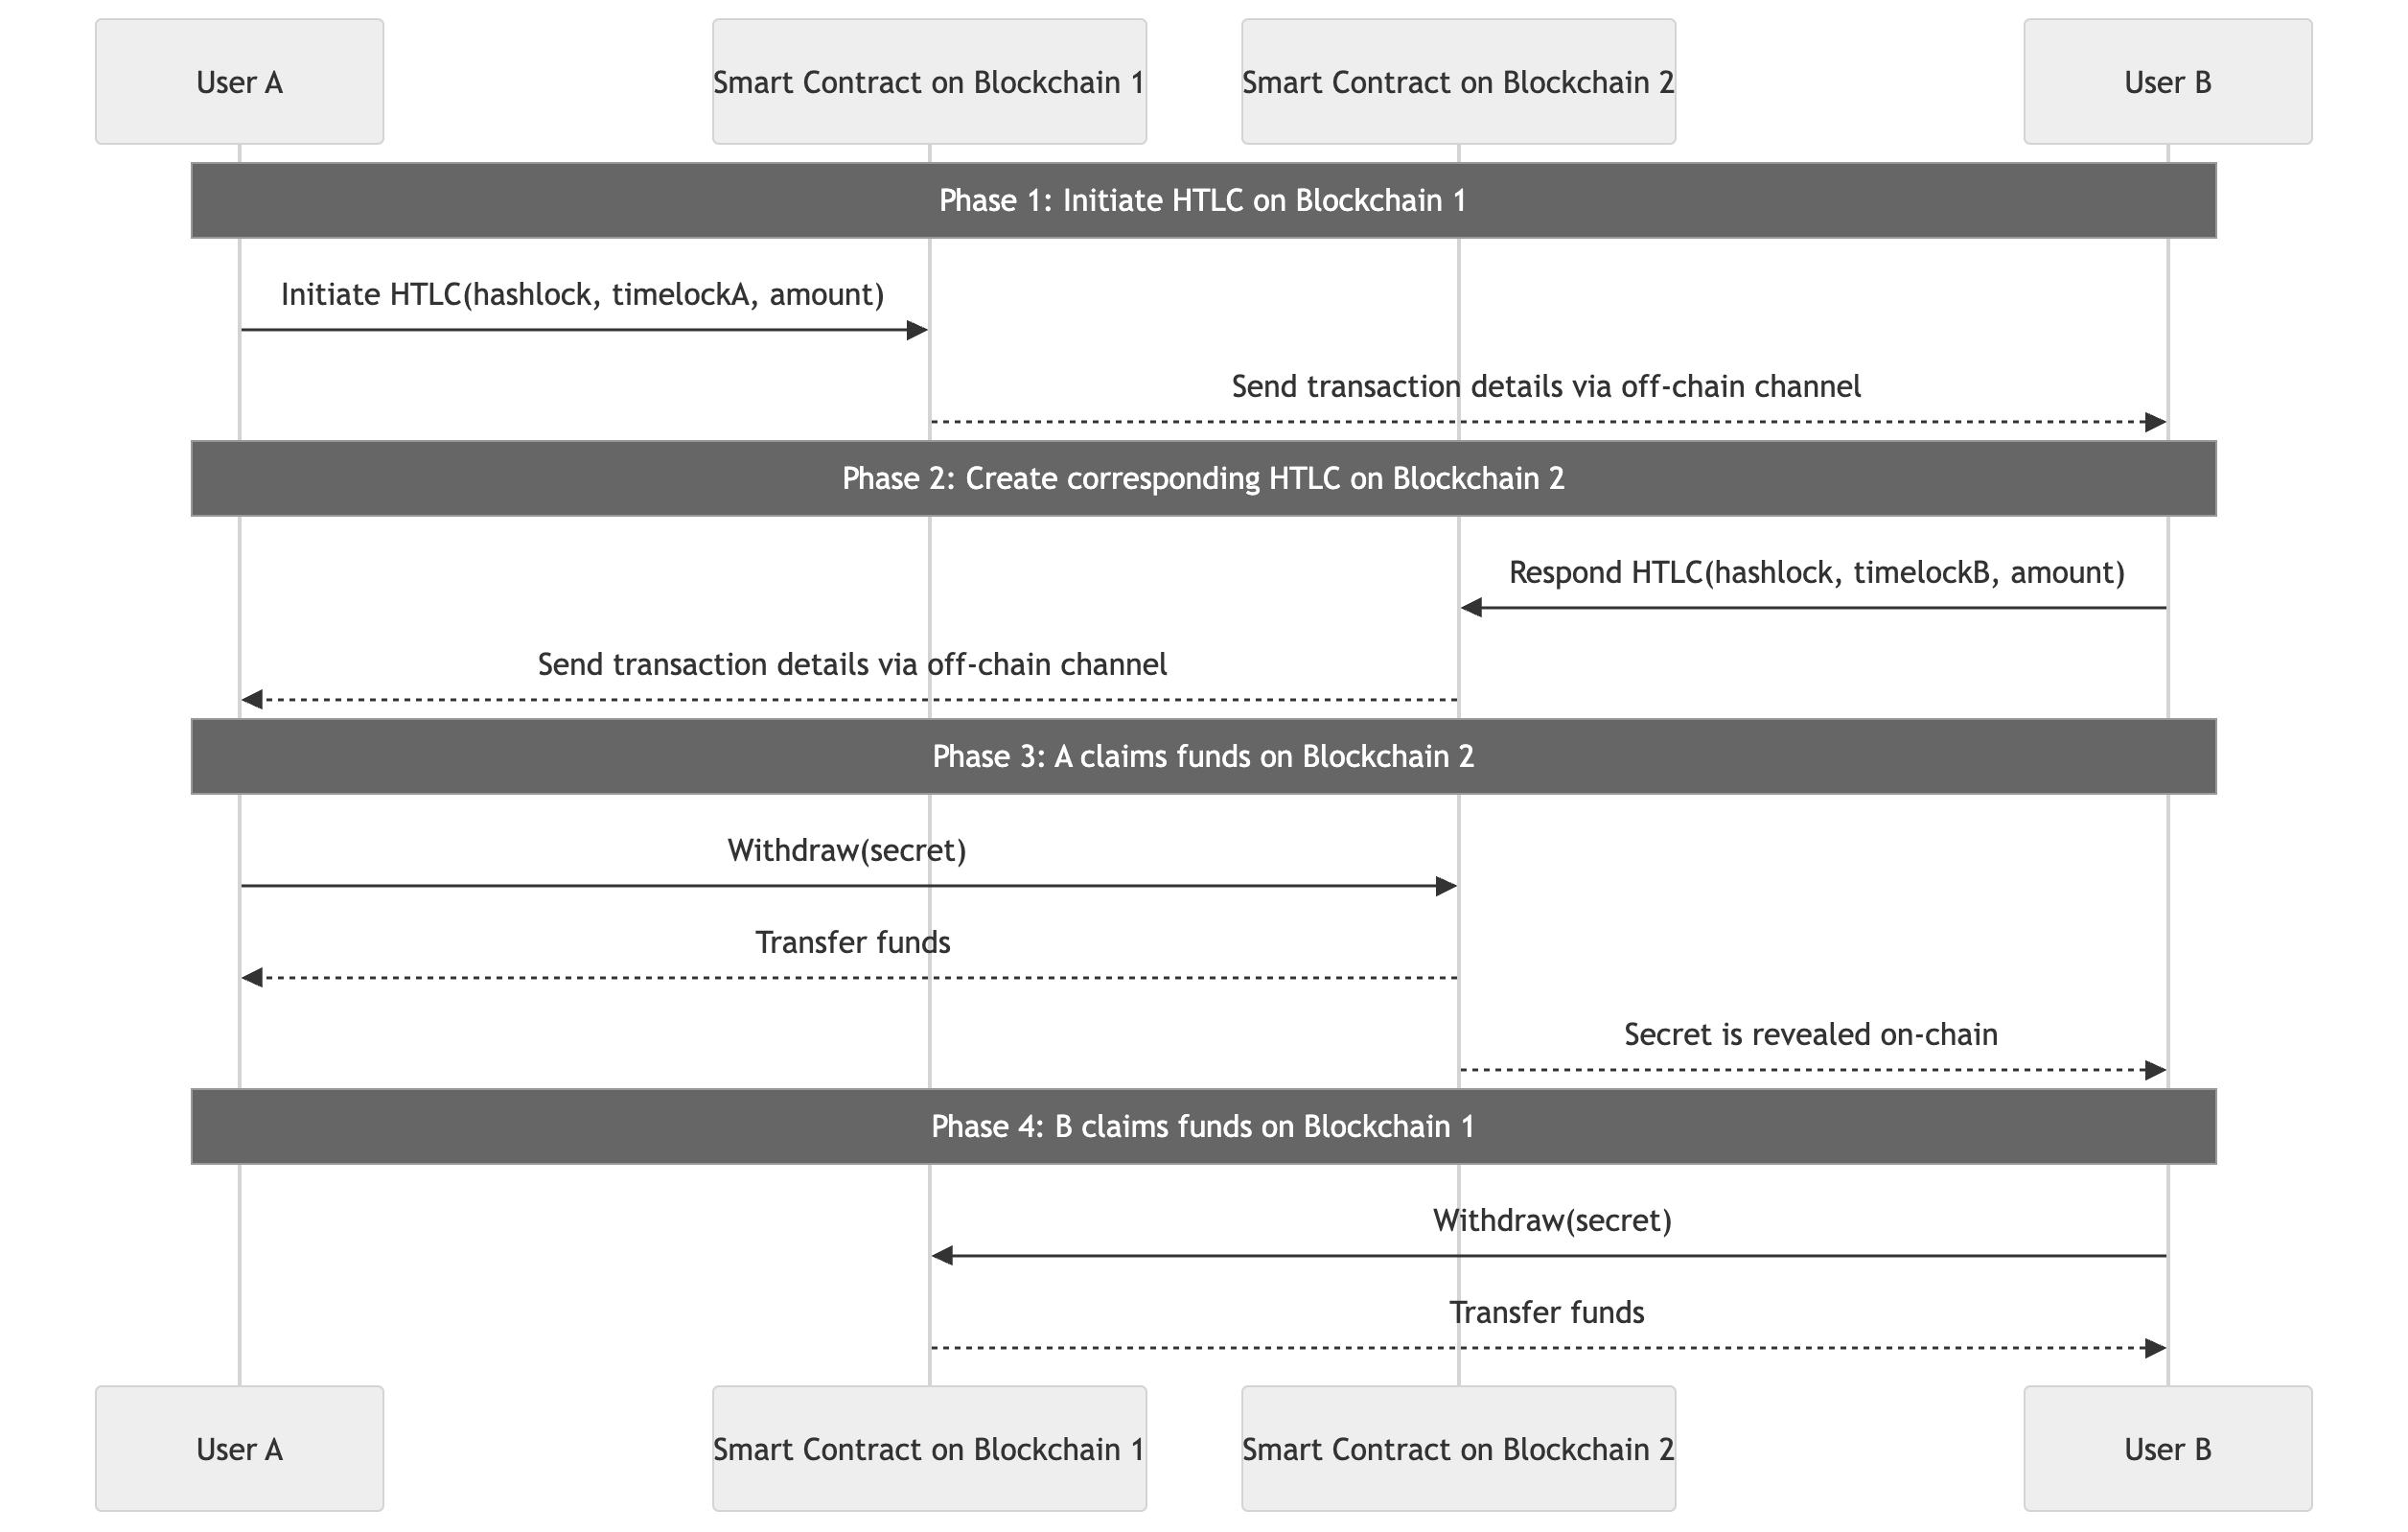
\includegraphics[width=\linewidth]{figures/c3/htlc-sequence}
  \caption{Biểu đồ tuần tự thuật toán HTLC giữa hai bên trên hai
  chuỗi}
\end{figure}

\subsubsection*{Multi-fill HTLC: thiết kế trong OceanLink}

HTLC chuẩn giả định mỗi hợp đồng tương ứng với \emph{một} cặp gửi–nhận.
Với matching theo vòng (cycle netting), trên cùng một chuỗi nguồn có
thể có nhiều người nhận khác nhau cần được thanh toán cùng một lúc, mỗi
người ứng với một hashlock riêng. Để giảm chi phí gas và đơn giản hoá
việc điều phối, OceanLink mở rộng HTLC theo hướng đa nhánh: mỗi
\textbf{Order} (đơn) chứa một hoặc nhiều \textbf{Fill} (nhánh thanh
toán). Cấu trúc dữ liệu chính được tóm tắt như sau:

\begin{itemize}
  \item \textbf{Order}: đại diện cho khoản tiền được \emph{một}
    người gửi khoá vào hợp đồng. Bao gồm: địa chỉ người gửi, token, tổng
    số tiền đã nạp, số tiền còn lại chưa được rút, thời gian khoá
    (\texttt{timelock}), trạng thái (\texttt{OPEN}/\texttt{REFUNDED}) và
    số lượng nhánh (\texttt{fillCount}).
  \item \textbf{Fill}: đại diện cho \emph{một} nhánh thanh toán bên
    trong order. Bao gồm: địa chỉ người nhận, số tiền của nhánh, hashlock
    và cờ \texttt{claimed}.
\end{itemize}

Một cấu trúc Order – Fill cho phép một giao dịch khoá tiền duy nhất phục
vụ nhiều cặp gửi–nhận, mỗi cặp được mở khoá độc lập bằng preimage tương
ứng.

\subsubsection*{Ba thao tác chính}

Hợp đồng cung cấp ba thao tác bên ngoài, tương ứng với ba pha của vòng
đời một order:

\paragraph{(1) \texttt{newOrder}.} Tạo order và đồng thời tạo toàn bộ
fill bên trong nó. Tham số gồm token, tổng số tiền, timelock và ba
mảng song song \texttt{receivers}, \texttt{amounts}, \texttt{hashlocks}.
Hợp đồng kiểm tra:

\begin{itemize}
  \item Token khác địa chỉ không, tổng số tiền dương, timelock thuộc
    tương lai.
  \item Ba mảng có cùng độ dài và không rỗng.
  \item Mỗi receiver khác địa chỉ không, mỗi amount dương.
  \item Tổng \texttt{amounts} không vượt quá số token thực sự nhận
    được sau khi gọi \texttt{transferFrom} (tính cả token có cơ chế
    \emph{fee-on-transfer}).
\end{itemize}

Sau khi xác thực, hợp đồng tăng định danh \texttt{nextOrderId}, ghi lại
order, sinh các fill và phát các sự kiện \texttt{OrderCreated} cùng
\texttt{FillCreated}. Phần token dư (\emph{dust}) — nếu tổng các fill
nhỏ hơn lượng thực sự nhận — được trả lại cho người gửi.

OceanLink cho phép một địa chỉ \emph{admin} đã được whitelist tạo order
\emph{thay mặt} một người dùng khác qua tham số \texttt{onBehalfOf}.
Tính năng này được Orchestrator sử dụng để gom nhiều fill cùng chuỗi
vào một giao dịch duy nhất, giúp tiết kiệm gas.
Khi \texttt{onBehalfOf} khác \texttt{msg.sender}, hợp đồng yêu cầu
\texttt{msg.sender} thuộc danh sách admin và token được kéo từ địa chỉ
\texttt{onBehalfOf}.

\paragraph{(2) \texttt{withdraw}.} Người nhận của một fill cụ thể (hoặc
một admin) cung cấp preimage để rút phần tiền của mình. Hợp đồng kiểm
tra:

\begin{itemize}
  \item Order tồn tại, đang ở trạng thái \texttt{OPEN}.
  \item Trừ khi cờ bất biến \texttt{allowWithdrawAfterExpiry} được bật
    lúc deploy, không cho rút sau \texttt{timelock}.
  \item Fill chưa từng được claim trước đó.
  \item $\mathcal{H}(\text{preimage}) = \text{hashlock}$, với
    $\mathcal{H}$ là hàm \texttt{sha256} của Solidity.
\end{itemize}

Theo nguyên tắc Checks–Effects–Interactions, hợp đồng đặt
\texttt{fill.claimed = true} và giảm \texttt{order.remainingAmount}
\emph{trước} khi gọi \texttt{safeTransfer} chuyển token cho người nhận.
Modifier \texttt{nonReentrant} cộng với mẫu CEI loại bỏ rủi ro tấn công
re-entrancy.

\paragraph{(3) \texttt{refund}.} Sau khi \texttt{timelock} hết hạn,
người gửi (hoặc admin) có thể gọi \texttt{refund} để lấy lại toàn bộ
phần tiền chưa được claim. Hợp đồng cập nhật trạng thái sang
\texttt{REFUNDED} và đặt \texttt{remainingAmount} về 0 trước khi chuyển
token. Đây là \emph{liveness escape hatch}: nếu vì bất kỳ lý do gì
preimage không được công bố trong thời gian khoá, tài sản không bị
khoá vĩnh viễn.

\subsubsection*{Thanh toán nguyên tử cho một vòng nhiều bên}

Để minh hoạ cách multi-fill HTLC bảo đảm tính nguyên tử cho một vòng
khớp lệnh nhiều bên, xét vòng có ba bên $A \to B \to C \to A$, mỗi
bên gửi USDC trên chuỗi nguồn của mình tới bên kế tiếp:

\begin{enumerate}
  \item Orchestrator gom các nhánh cùng chuỗi vào các \emph{order
    consolidated}. Một order trong số đó được chỉ định là \emph{order
    chủ tịch} (presiding); những order còn lại là \emph{order phản hồi}
    (responding).
  \item Order chủ tịch sinh tươi các bí mật $s_i$ và publish các
    hashlock $h_i = \mathcal{H}(s_i)$ qua sự kiện \texttt{FillCreated}.
  \item Các order phản hồi \emph{tái sử dụng} các hashlock $h_i$ này
    khi tạo HTLC trên các chuỗi khác. Như vậy mọi nhánh thuộc cùng
    một cặp đối ứng đều bị khoá bởi cùng một bí mật.
  \item Sau khi tất cả các HTLC đã có mặt trên chuỗi, Orchestrator gọi
    \texttt{withdraw} với các preimage tương ứng. Vì các preimage
    được công khai trên chuỗi qua sự kiện
    \texttt{FillWithdrawn}, mọi bên nhận ở mọi chuỗi đều có thể quan
    sát và sử dụng để rút phần của mình.
  \item Nếu bước nào đó thất bại, các HTLC chưa được rút sẽ tự động
    được hoàn lại sau \texttt{timelock}; không có nhánh nào bị mất
    vĩnh viễn.
\end{enumerate}

Tính chất an toàn cốt lõi của thiết kế: \emph{biết một preimage
$s_i$ là điều kiện đủ để mở khoá tất cả các nhánh chia sẻ
$h_i$ trên mọi chuỗi}. Cộng với cơ chế refund-after-timelock, hệ
thống thoả tính chất \textbf{liveness} (tài sản luôn về tay đúng
chủ hoặc trở về người gửi) và \textbf{safety} (không có trạng thái mà
một bên mất tài sản trong khi bên đối ứng vẫn được nhận).

\subsubsection*{Một số cân nhắc kỹ thuật}

\begin{itemize}
  \item \textbf{Hàm băm.} Sử dụng \texttt{sha256} thay vì
    \texttt{keccak256} để dễ đồng bộ với các nguyên thủy của các
    blockchain non-EVM trong tương lai (Bitcoin, Cosmos), nơi
    \texttt{sha256} là tiêu chuẩn de facto.
  \item \textbf{Bảo vệ re-entrancy.} Mọi hàm thay đổi trạng thái
    đều được khoanh bằng modifier \texttt{nonReentrant} của OpenZeppelin
    và tuân thủ mẫu CEI.
  \item \textbf{Token có fee-on-transfer.} Hợp đồng đo lượng token
    \emph{thực sự nhận được} bằng cách so sánh
    \texttt{balanceOf} trước và sau khi gọi \texttt{transferFrom},
    rồi yêu cầu tổng các fill không vượt quá số đó. Phần dư được
    trả lại người gửi.
  \item \textbf{Granularity của timelock.} Tham số
    \texttt{TIME\_LOCK} mặc định 10 phút (cấu hình qua biến môi
    trường) là sự cân bằng giữa thời gian đủ để Orchestrator hoàn
    tất nhiều giao dịch trên ba chuỗi và thời gian không quá lâu
    để khoá tài sản người dùng nếu sự cố xảy ra.
\end{itemize}

% =============================================================================
% Draft mục 3.3.2 — API Gateway
% =============================================================================

\subsection{API Gateway}
\label{sec:api-gateway}

API Gateway là điểm vào duy nhất của backend. Tất cả các tương tác giữa frontend và phần lõi off-chain (orderbook, matching, execution) đều đi qua tầng này. Cài đặt dựa trên Fastify --- một web framework Node.js có hiệu năng cao và schema validation tích hợp --- chạy như một plugin trong cùng tiến trình với matching scheduler và các engine khác.

\subsubsection{Cấu trúc route}

Các endpoint được nhóm theo khu vực tương ứng với bốn module chính. Nhóm \texttt{/api/intent} phục vụ submit intent mới, truy vấn trạng thái intent và mở stream SSE lifecycle. Nhóm \texttt{/api/orchestrator} phục vụ truy vấn \texttt{ExecutionRecord} của một matchId. Hai nhóm \texttt{/api/bridge} và \texttt{/api/htlc} cho phép gọi trực tiếp các thao tác on-chain (tạo HTLC, withdraw, refund) bỏ qua matching engine, chủ yếu phục vụ script vận hành và testing thủ công. Cuối cùng, nhóm \texttt{/api/approval} quản lý USDC approval cho LP wallet.

\subsubsection{Vai trò trong bốn nhóm thao tác}

\subsubsection*{Submit intent}

\texttt{POST /api/intent} nhận body JSON với các trường \texttt{srcChain}, \texttt{desChain}, \texttt{amount}, \texttt{deadline}, \texttt{userAddress}, và tuỳ chọn \texttt{incentiveFee}. Hàm \texttt{validateIntent} thực hiện các kiểm tra:

\begin{itemize}
    \item Hai chuỗi nguồn--đích khác nhau và cùng được hỗ trợ.
    \item \texttt{amount} là số nguyên dương dạng chuỗi, không tràn.
    \item \texttt{deadline} thuộc tương lai (so với \texttt{Math.floor(Date.now() / 1000)}).
    \item \texttt{userAddress} đúng định dạng EVM.
\end{itemize}

Nếu hợp lệ, gateway sinh \texttt{orderId} (UUID), đặt \texttt{status = QUEUED}, gọi \texttt{orderStore.add()} và phản hồi \texttt{201 Created} kèm \texttt{orderId}. Các route truy vấn (\texttt{GET /api/intent/:id}) đọc trực tiếp từ in-memory OrderStore, tận dụng tính chất tra cứu $O(1)$ của primary index.

\subsubsection*{Stream lifecycle (SSE)}

\texttt{GET /api/intent/:orderId/events} mở một kết nối Server-Sent Events. Handler đăng ký một listener trên \texttt{orderEvents}, lọc theo \texttt{orderId}, và push các \texttt{OrderEvent} xuống client ở định dạng \texttt{text/event-stream}. Khi client ngắt kết nối, listener được tháo gỡ để tránh rò bộ nhớ.

\subsubsection*{Truy vấn execution}

\texttt{GET /api/orchestrator/execution/:matchId} trả về \texttt{ExecutionRecord} cho một match đã (hoặc đang) thực thi. Dữ liệu gồm order chủ tịch (chainKey, orderId, secrets), các responding withdraw, và trạng thái \texttt{pending}/\texttt{done}/\texttt{error}. Endpoint này được frontend dùng để hiển thị giao diện kết quả cuối cùng (txHash trên các chuỗi, người nhận, số tiền).

\subsubsection*{Thao tác on-chain trực tiếp}

Các route dưới \texttt{/api/bridge}, \texttt{/api/htlc}, \texttt{/api/approval} đóng gói các phép nguyên thủy của \texttt{BridgeService}: tạo HTLC, rút, hoàn lại, approve. Chúng \emph{không} đi qua matching engine; đây là kênh thoát hiểm để thực hiện các thao tác đặc thù như debugging, hoặc bridge thủ công khi muốn kiểm thử HTLC mà không cần matching cycle.

\subsubsection{CORS và xác thực}

CORS được mở cho \texttt{FRONTEND\_URL} (cấu hình qua biến môi trường, mặc định \texttt{http://localhost:3000}) với \texttt{credentials: true}. Trong scope MVP, hệ thống không có authentication và rate limiting; bất kỳ ai biết URL đều có thể submit intent. Đây là quyết định có chủ đích để giảm phạm vi của luận văn. Trong production, các tầng xác thực (API key, signature-based authentication, hoặc EIP-4361 Sign-In with Ethereum) sẽ được thêm giữa frontend và gateway.

\subsubsection{Vai trò Risk engine trong intention diagram}

Trong sơ đồ kiến trúc dự kiến, một module \emph{Risk engine} riêng biệt được vẽ giữa API Gateway và Orderbook để kiểm tra các thuộc tính rủi ro (sender bị blocklist, intent vi phạm chính sách, ...). Trong cài đặt hiện tại, vai trò này được hợp nhất vào hàm \texttt{validateIntent} ở route handler, đủ cho scope MVP và testnet. Việc tách Risk engine thành module độc lập kèm các kiểm tra phức tạp như sanction screening hay AML scoring được liệt kê ở Future Work.

% =============================================================================
% Draft mục 3.3.3 — Order Book (OrderStore)
% =============================================================================

\subsection{Order Book (OrderStore)}
\label{sec:order-book}

\texttt{OrderStore} là sổ lệnh (orderbook) của hệ thống, nơi các intent đang active được lưu trữ giữa thời điểm người dùng gửi và thời điểm Matching Engine khớp được chúng. Thiết kế của OrderStore phản ánh một quyết định kiến trúc quan trọng: tách \emph{nguồn sự thật lúc chạy} (runtime source of truth) khỏi \emph{lưu trữ bền} (durable storage), dùng cơ chế write-through cache để vừa giữ độ trễ thấp cho matching tick, vừa đảm bảo dữ liệu không mất khi tiến trình khởi động lại.

\subsubsection{Hai tầng dữ liệu}

\subsubsection*{Tầng trong bộ nhớ (in-memory)}

Tầng này là các cấu trúc JavaScript \texttt{Map} sống trong tiến trình Node của backend, gồm ba cấu trúc chính:

\begin{itemize}
    \item \emph{Primary index} dạng \texttt{Map<orderId, IntentOrder>} cho tra cứu một order theo định danh trong $O(1)$.
    \item \emph{Pair index} dạng \texttt{Map<"src-des", Set<orderId>>} cho tra cứu nhanh tập order đang hoạt động theo cặp chuỗi nguồn--đích trong $O(1)$. Pair index chỉ chứa các order \texttt{QUEUED} hoặc \texttt{PARTIAL}; khi một order chuyển sang \texttt{MATCHED} hoặc \texttt{EXPIRED}, pair index được xoá tham chiếu tương ứng để Matching Engine không phải lọc lại.
    \item \emph{Match log} dạng mảng \texttt{MatchResult[]} append-only, lưu lịch sử tất cả các sự kiện match đã phát sinh.
\end{itemize}

\subsubsection*{Tầng bền vững (Postgres)}

Tầng này là cơ sở dữ liệu quan hệ Postgres chạy trong tiến trình riêng biệt, được truy cập qua Drizzle ORM, với ba bảng tương ứng:

\begin{itemize}
    \item \texttt{intent\_orders}: mỗi dòng là một \texttt{IntentOrder}. Số lượng được lưu dạng \texttt{text} để giữ chính xác tuyệt đối (USDC dùng 6 chữ số thập phân, lớp matching xử lý chuỗi số nguyên bất kỳ).
    \item \texttt{match\_results}: bảng nhật ký append-only của các sự kiện match. Các trường \texttt{cycles} và \texttt{raw\_cycles} được lưu dạng JSONB do hệ thống không cần truy vấn vào nội dung.
    \item \texttt{executions}: lưu trạng thái thực thi mỗi \texttt{matchId}, được cập nhật theo thời gian thực khi Orchestrator chuyển trạng thái \texttt{pending} $\rightarrow$ \texttt{done|error}.
\end{itemize}

\subsubsection{Mô hình write-through}

Mọi thao tác mutating trên OrderStore đều theo trình tự hai bước. Trước tiên, hệ thống cập nhật cấu trúc trong bộ nhớ \emph{đồng bộ} (synchronous) để các thành phần đọc tiếp theo (Matching Engine, các route đọc) nhìn thấy giá trị mới ngay lập tức. Sau đó, hệ thống phát một thao tác ghi tương ứng vào Postgres theo kiểu \emph{fire-and-forget}: tạo Promise, không await, gắn handler \texttt{logDbError} cho trường hợp lỗi.

Mục tiêu thiết kế là không để vòng lặp matching (chu kỳ 1\,s) bị chặn bởi I/O cơ sở dữ liệu. Đánh đổi đi kèm là nếu tiến trình bị crash giữa bước 1 và bước 2, trạng thái trong bộ nhớ và Postgres có thể lệch nhau trong một khoảng ngắn — chấp nhận được ở giai đoạn MVP. Phương án nâng cấp được liệt kê ở mục Future Work là chuyển sang \emph{outbox pattern}, tức append event vào một bảng riêng trong cùng một transaction với việc thay đổi trạng thái, rồi để một consumer riêng đọc bảng đó.

\subsubsection{Hydration on boot}

Vì in-memory không phải durable, nó phải được \emph{rehydrate} (tái xây dựng) từ Postgres mỗi khi tiến trình khởi động. Phương thức \texttt{OrderStore.hydrate()} chạy trước khi \texttt{MatchScheduler} bắt đầu tick, gồm hai bước. Đầu tiên là \texttt{SELECT * FROM intent\_orders} để đọc toàn bộ order, dựng lại primary index và pair index; chỉ các order \texttt{QUEUED} hoặc \texttt{PARTIAL} được đưa vào pair index, vì pair index chỉ đại diện các order còn ứng cử để match. Tiếp theo là \texttt{SELECT * FROM match\_results ORDER BY matched\_at} để đọc nhật ký match và append theo thứ tự thời gian.

Hydration được \emph{await} trong \texttt{start()} của entrypoint backend; nếu hydration thất bại, tiến trình crash thay vì bắt đầu chạy với trạng thái rỗng. Đây là lựa chọn an toàn vì rỗng có thể vô tình bỏ mất các order còn pending hoặc các execution chưa hoàn tất.

\subsubsection{Vai trò trong sơ đồ phụ thuộc}

OrderStore là singleton của module \texttt{matching/store/orderStore} và được chia sẻ bởi hai nhóm consumer chính. Phía API Gateway gọi \texttt{add()} khi nhận \texttt{POST /api/intent} và gọi \texttt{get()} khi nhận các route truy vấn. Phía MatchingService gọi \texttt{getActiveOrders()}, \texttt{getByPair()}, \texttt{update()}, \texttt{removeFromPairIndex()}, \texttt{addMatchResult()}, \texttt{expireStale()}.

Nói cách khác, OrderStore đóng vai trò bus dữ liệu nội bộ: \emph{mọi thay đổi trạng thái orderbook đi qua nó}, và mọi việc ghi xuống Postgres do \emph{một mình OrderStore} chịu trách nhiệm. Nhờ đó các thành phần khác (MatchingService) không cần biết về sự tồn tại của Postgres — một dạng dependency inversion đơn giản.

% =============================================================================
% Draft mục 3.3.4 — Matching Engine
% Đặt trong c3/ và \input{} vào c3_chapter.tex sau khi rà soát.
% =============================================================================

\subsection{Matching Engine}
\label{sec:matching-engine}

Matching Engine là hạt nhân của lớp Netting: nó nhận đầu vào là tập
intent đang chờ, mô hình hoá chúng thành một đồ thị có hướng có trọng
số, rồi tìm các vòng (cycle) cho phép \emph{nhiều bên cùng nhận tài sản
mà không cần một bể thanh khoản trung gian}. Đây là cơ chế làm cho
OceanLink có thể khớp một phần lớn nhu cầu chuyển bridge \emph{P2P} —
khác với các bridge truyền thống vốn dựa trên locked liquidity hoặc
mint–burn.

Phần này mô tả ba thành phần của engine: cấu trúc dữ liệu, vòng lặp
điều phối (\texttt{MatchingService} + \texttt{MatchScheduler}), và
trọng tâm là thuật toán giảm chu trình (cycle-reduction algorithm).

\subsubsection*{Mô hình hoá: orderbook là một đồ thị có hướng}

Tại một thời điểm bất kỳ, tập các intent đang ở trạng thái
\texttt{QUEUED} hoặc \texttt{PARTIAL} được biểu diễn thành một đồ thị
có hướng có trọng số $G = (V, E)$:

\begin{itemize}
  \item Mỗi đỉnh $v \in V$ là một \emph{chuỗi} (chain). Trong scope
    luận văn, $|V| = 3$ tương ứng Ethereum Sepolia, Arbitrum Sepolia,
    Base Sepolia.
  \item Mỗi cạnh có hướng $e = (u, v, w) \in E$ là một
    intent: $u$ là chuỗi nguồn, $v$ là chuỗi đích, $w$ là
    \emph{trọng số hiệu dụng} của intent — bằng số lượng USDC cộng
    với phần \texttt{incentiveFee} (nếu có).
  \item Đồ thị là multigraph có hướng (cho phép nhiều cạnh giữa
    cùng một cặp đỉnh): trên cùng cặp $(u, v)$ có thể có nhiều
    intent của nhiều người dùng khác nhau.
\end{itemize}

Một \emph{chu trình có hướng} (directed cycle) trong $G$ tương ứng với
một vòng đối ứng: dãy intent $u_1 \to u_2 \to \dots \to u_k \to u_1$
sao cho tổng tài sản chuyển vào và chuyển ra của mỗi chuỗi cân bằng
nhau, do đó có thể thanh toán nguyên tử. Hình \ref{fig:matching-graph}
minh hoạ một snapshot điển hình của orderbook dưới dạng đồ thị có
hướng có trọng số: mỗi đỉnh là một chuỗi, mỗi cạnh là một intent với
trọng số là số USDC hiệu dụng, và các chu trình trong đồ thị chính là
ứng viên cho việc khớp lệnh.

\begin{figure}[H]
  \centering
  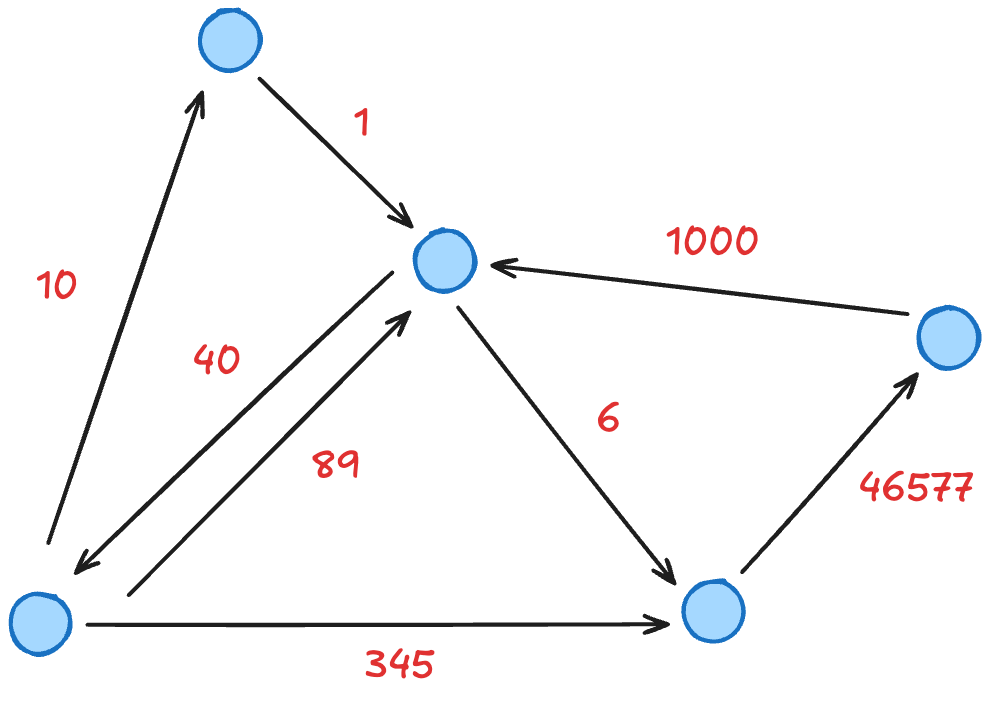
\includegraphics[width=0.85\linewidth]{figures/c3/graph}
  \caption{Mô hình hoá orderbook thành đồ thị có hướng có trọng số}
  \label{fig:matching-graph}
\end{figure}

\subsubsection*{Vòng lặp điều phối}

Hai thành phần cộng tác để chạy việc khớp lệnh định kỳ:

\paragraph{\texttt{MatchScheduler}} là một vòng lặp dựa trên
\texttt{setInterval} với chu kỳ mặc định 5\,s (cấu hình qua
\texttt{MATCH\_INTERVAL\_MS}). Cứ mỗi 5 giây, scheduler gom toàn bộ
intent đang sống thành một \emph{batch} và gọi
\texttt{MatchingService.runTick()} để tìm các chu trình bù trừ trên
batch đó; cửa sổ 5 giây là sự cân bằng giữa việc cho đủ thời gian để
nhiều intent đối ứng cùng tích luỹ trong cùng một batch (tăng khả
năng tạo cycle) và việc giữ độ trễ chấp nhận được cho người dùng. Vì
Node.js là single-threaded, một cờ boolean \texttt{isRunning} là đủ
để ngăn các tick chồng lên nhau khi một tick chưa kịp hoàn tất;
không cần mutex.

\paragraph{\texttt{MatchingService.runTick()}} thực thi một tick:

\begin{enumerate}
  \item \textbf{Hết hạn.} Quét \texttt{OrderStore}, đánh dấu các order
    có \texttt{deadline} đã trôi qua thành \texttt{EXPIRED} và xoá khỏi
    pair index.
  \item \textbf{Snapshot.} Lấy mảng các order còn hoạt động
    (\texttt{QUEUED} hoặc \texttt{PARTIAL}).
  \item \textbf{Build graph.} Chuyển snapshot thành tập cạnh và xác
    định số đỉnh.
  \item \textbf{Tìm chu trình.} Gọi
    \texttt{runAlgorithm($n$, edges, $x$)} — chính là thuật toán giảm
    chu trình mô tả ở phần sau.
  \item \textbf{Translate.} Dịch các chu trình bắt được thành các
    đối tượng \texttt{MatchResult}: cập nhật trạng thái mỗi order
    bị ảnh hưởng thành \texttt{MATCHED} (đã được match toàn bộ) hoặc
    \texttt{PARTIAL} (mới được match một phần).
  \item \textbf{Persist.} Append \texttt{MatchResult} vào nhật ký match
    của \texttt{OrderStore} (qua đó được mirror sang Postgres).
  \item \textbf{Hand-off.} Trả \texttt{TickStats} cho scheduler;
    scheduler chuyển danh sách \texttt{MatchResult} sang Orchestrator
    để thực thi on-chain.
\end{enumerate}

\subsubsection*{Thuật toán giảm chu trình (cycle-reduction)}

Cốt lõi thuật toán nằm ở bước 4: tìm các chu trình \emph{đáng để khớp}
trong $G$ và đồng thời cập nhật $G$ để phản ánh phần đã được tiêu thụ.
Về mặt lý thuyết, bài toán \emph{tối đa hoá tổng khối lượng được khớp}
trên một đồ thị bất kỳ là NP-hard nếu yêu cầu nghiệm tối ưu toàn cục.
Do hệ thống cần chạy thời gian thực với chu kỳ 5\,s, OceanLink chọn
một chiến lược tham lam dựa trên DFS với một ngưỡng chấp nhận được.

\paragraph{Tham số ngưỡng $x \in [0, 1]$.} Cấu hình qua
\texttt{MATCH\_THRESHOLD} (mặc định $0.3$). Một chu trình $C$ chỉ
được khớp nếu

\[
  \mathrm{ratio}(C) \;=\; \frac{\min_{e \in C} w(e)}{\max_{e \in C} w(e)} \;>\; x.
\]

Ý nghĩa: tỉ số $\mathrm{ratio}$ đo độ \emph{cân bằng} của chu trình.
Khi $\mathrm{ratio} = 1$, mọi cạnh có cùng trọng số, vòng được khớp
hoàn toàn. Khi $\mathrm{ratio}$ rất nhỏ, chu trình có một cạnh quá
yếu so với các cạnh còn lại — chỉ một phần rất nhỏ tài sản có thể
được khớp, phần còn dư phải xếp hàng tiếp; chi phí gas khi thực thi
sẽ không đủ bù lại lợi ích. Ngưỡng $x$ là cơ chế tránh khớp các chu
trình "lệch" như vậy.

\paragraph{Bộ khung DFS ba màu.} Việc tìm một chu trình bất kỳ trong
đồ thị có hướng được thực hiện bằng DFS với ba màu:

\begin{itemize}
  \item \textbf{trắng} (0): đỉnh chưa được duyệt.
  \item \textbf{xám} (1): đỉnh đang nằm trên ngăn xếp DFS hiện tại.
  \item \textbf{đen} (2): đỉnh đã duyệt xong, mọi hậu duệ đã được
    khám phá.
\end{itemize}

Khi DFS phát hiện một cạnh trỏ đến đỉnh \emph{xám} (back-edge), một
chu trình tồn tại. Thuật toán duy trì một ngăn xếp các cạnh đang ở
trên đường DFS hiện tại, từ đó tái dựng chu trình bằng cách trích
phần đuôi của ngăn xếp tính từ cạnh nối đến đỉnh xám đó.

\paragraph{Bước cập nhật.} Sau khi xác định được một chu trình $C$
với $\mathrm{ratio}(C) > x$, thuật toán thực hiện ba việc:

\begin{enumerate}
  \item \textbf{Snapshot.} Lưu lại bản sao bất biến của các cạnh
    trong $C$ kèm trọng số tại thời điểm khớp. Snapshot này là dữ
    liệu nguyên thuỷ để Orchestrator dựng lại các \texttt{SendAction}.
  \item \textbf{Loại cạnh tối thiểu.} Cạnh có trọng số $w_{\min} =
    \min_{e \in C} w(e)$ bị xoá khỏi đồ thị (intent tương ứng được
    đánh dấu \texttt{MATCHED}, đã sử dụng trọn).
  \item \textbf{Trừ trọng số.} Mọi cạnh khác trong $C$ bị giảm
    trọng số đi đúng $w_{\min}$ — phần "đã tiêu" trên các intent
    còn lại. Các intent đó chuyển sang \texttt{PARTIAL} với phần
    còn lại trong queue chờ tick sau.
\end{enumerate}

Sau bước cập nhật, đồ thị mới có ít hơn ít nhất một cạnh; thuật toán
lặp lại từ đầu — DFS lại trên đồ thị mới — cho đến khi không còn chu
trình nào hoặc chu trình tìm được không thoả ngưỡng.

\paragraph{Mã giả tổng quát.}

\begin{verbatim}
function runAlgorithm(n, edges, x):
    capturedCycles <- []
    repeat:
        C <- findOneCycle(n, edges)         // DFS three-colour
        if C is empty: break
        let w_min = min(edge.w for edge in C)
        let w_max = max(edge.w for edge in C)
        if w_min / w_max <= x: break
        capturedCycles.append( snapshotOf(C) )
        remove the edge of weight w_min from edges
        for each remaining edge e in C:
            e.w <- e.w - w_min
    return capturedCycles
\end{verbatim}

\paragraph{Đảm bảo dừng (termination).} Mỗi vòng lặp loại đúng một
cạnh khỏi đồ thị, do $|E|$ luôn giảm sau mỗi lần lặp thành công.
Thuật toán dừng tối đa sau $|E|$ vòng lặp, vì vậy độ phức tạp là
$O(|E| \cdot |V| \cdot |E|) = O(|V| \cdot |E|^2)$ — DFS có chi phí
$O(|V| + |E|)$ và được lặp tối đa $|E|$ lần. Trong thực tế $|V|$ rất
nhỏ (số chuỗi) và $|E|$ giới hạn bởi số intent đang sống, nên chi phí
là chấp nhận được.

\paragraph{Tham lam và không tối ưu.} Thuật toán không bảo đảm tìm
được chu trình tốt nhất theo bất kỳ tiêu chí nào (tổng khối lượng,
tổng phí incentive, độ dài chu trình ngắn nhất). Đây là sự đánh đổi
có chủ đích:

\begin{itemize}
  \item \emph{Đơn giản, dễ kiểm chứng}: thuật toán chỉ phụ thuộc vào
    DFS chuẩn và phép so sánh trọng số, dễ test và dễ debug.
  \item \emph{Latency thấp}: hoàn tất trong vài mili-giây ngay cả khi
    có hàng chục intent.
  \item \emph{Đảm bảo "an toàn về kinh tế"}: ngưỡng $x$ ngăn
    việc khớp các vòng quá lệch có chi phí gas cao so với lợi ích.
\end{itemize}

Việc nâng cấp lên thuật toán tối ưu (ví dụ negative-cycle Bellman-Ford
trên một biến đổi của đồ thị, hay LP relaxation) được liệt kê trong
phần Future Work.

\subsubsection*{Ví dụ minh hoạ}

Xét đồ thị bốn cạnh: $0 \to 1$ trọng số 10, $1 \to 0$ trọng số 2,
$1 \to 2$ trọng số 8, $2 \to 1$ trọng số 4 và $x = 0.1$:

\begin{enumerate}
  \item \textbf{Vòng lặp 1.} DFS tìm thấy chu trình $0 \to 1 \to 0$.
    $\mathrm{ratio} = 2/10 = 0.2 > 0.1$ $\rightarrow$ khớp. Snapshot
    $[(0\to1, 10), (1\to0, 2)]$ được lưu. Cạnh $1 \to 0$ bị xoá.
    Cạnh $0 \to 1$ giảm còn 8.
  \item \textbf{Vòng lặp 2.} DFS tìm thấy chu trình $1 \to 2 \to 1$.
    $\mathrm{ratio} = 4/8 = 0.5 > 0.1$ $\rightarrow$ khớp. Snapshot
    $[(1\to2, 8), (2\to1, 4)]$ được lưu. Cạnh $2 \to 1$ bị xoá.
    Cạnh $1 \to 2$ giảm còn 4.
  \item \textbf{Vòng lặp 3.} Đồ thị còn lại $\{0\to1(8),\ 1\to2(4)\}$
    là acyclic; thuật toán dừng.
\end{enumerate}

Kết quả: hai chu trình được khớp trong cùng một tick. Hành vi này được
phủ trong test \texttt{algorithm.test.ts} và là cơ sở để Orchestrator
gom thành các order consolidated trên cùng chuỗi.

\subsubsection*{Liên kết với incentive fee}

\texttt{IntentOrder} cho phép người dùng kèm trường \texttt{incentiveFee}
\emph{tuỳ chọn}. Trọng số của cạnh không phải là số USDC nguyên gốc mà
là \emph{số tiền hiệu dụng}:

\[
  w(e) = \mathrm{amount}(e) + \mathrm{incentiveFee}(e).
\]

Hệ quả: các intent có incentive fee cao có cạnh nặng hơn, nên có nhiều
khả năng nằm trong chu trình thoả ngưỡng và được khớp trước. Đây là
một cơ chế đấu giá ngầm cho thứ tự ưu tiên match — không cần một sổ
giá riêng.

% =============================================================================
% Draft mục 3.3.6 — Execution Engine (Orchestrator + BridgeService)
% =============================================================================

\subsection{Execution Engine: Orchestrator và BridgeService}
\label{sec:execution-engine}

Khi Matching Engine sản sinh một \texttt{MatchResult} chứa các chu
trình đã được khớp về mặt logic, công việc còn lại là biến chu trình
đó thành các giao dịch trên chuỗi sao cho \emph{tài sản chỉ thực sự
chuyển nếu mọi nhánh trong chu trình đều thành công}. Đây là vai trò
của Execution Engine, được tách thành hai tầng: \textbf{Orchestrator}
chịu trách nhiệm lập kế hoạch và điều phối, và \textbf{BridgeService}
là tầng thấp gói gọn các tương tác cụ thể với hợp đồng HTLC trên từng
chuỗi.

\subsubsection*{Mô hình "presiding/responding"}

Một chu trình có thể chứa nhiều cạnh trên cùng một chuỗi (nhiều
intent có cùng chuỗi nguồn nhưng khác chuỗi đích, hoặc ngược lại).
Với HTLC chuẩn, mỗi cạnh sẽ là một giao dịch riêng — chi phí gas
cao và phải đồng bộ nhiều secret/hashlock. OceanLink tận dụng tính
chất multi-fill của HTLC (xem
\S\ref{sec:smart-contract-layer}) để \emph{gom} các cạnh cùng chuỗi
nguồn vào \emph{một} order với nhiều fill, giảm số giao dịch
cần phát.

Trong mỗi \texttt{MatchResult}, một order consolidated được Orchestrator
chọn làm \emph{order chủ tịch} (\texttt{presiding order}); các order
còn lại là \emph{order phản hồi} (\texttt{responding orders}).
Phân vai này quyết định ai sinh bí mật:

\begin{itemize}
  \item \textbf{Order chủ tịch} sinh các bí mật $s_i$ tươi (random
    256-bit) tại lúc tạo, và publish các hashlock
    $h_i = \mathrm{SHA256}(s_i)$ qua sự kiện \texttt{FillCreated}.
  \item \textbf{Các order phản hồi} \emph{không sinh bí mật mới}; thay
    vào đó, chúng tái sử dụng các $h_i$ đã có. Mỗi fill trong order
    phản hồi liên kết với đúng một fill trong order chủ tịch (qua
    chỉ số chu trình), do đó cùng chia sẻ một preimage.
\end{itemize}

Cấu trúc này là cốt lõi của tính nguyên tử: \emph{biết một preimage
$s_i$ là điều kiện đủ để mở khoá tất cả các fill chia sẻ
$h_i$ trên mọi chuỗi}. Khi order chủ tịch được rút bằng $s_i$, giá
trị $s_i$ trở thành công khai trên chuỗi — bất kỳ ai (Orchestrator
trong trường hợp này) cũng có thể dùng nó để rút các fill phản hồi
tương ứng trên các chuỗi khác.

\subsubsection*{Thuật toán \texttt{handleMatchResults}}

Orchestrator nhận một mảng \texttt{MatchResult} từ scheduler. Với
mỗi \texttt{MatchResult} (xử lý tuần tự để giữ thứ tự thời gian
matchId), thực hiện các bước sau:

\begin{enumerate}
  \item Đặt \texttt{ExecutionRecord} cho \texttt{matchId} sang
    \texttt{pending} và persist vào bảng \texttt{executions}.
  \item Trích các \emph{send action} từ chu trình
    (\texttt{extractSendActionsFromCycles}). Mỗi send action mô tả:
    cạnh nào, chuỗi nguồn nào, người gửi nào (địa chỉ ví), người
    nhận nào, số tiền bao nhiêu, thuộc chu trình nào.
  \item Gom các action có cùng \emph{chuỗi nguồn + người gửi} thành
    nhóm (\texttt{groupActionsByChainKey}); mỗi nhóm sẽ trở thành
    \emph{một} order multi-fill trên chuỗi đó.
  \item Chọn nhóm đầu tiên làm presiding, gọi
    \texttt{executePresidingOrder} $\rightarrow$ BridgeService.\texttt{createOrder}
    với cờ \texttt{isPresiding=true}. Kết quả: orderId trên chuỗi,
    txHash, danh sách $\{s_i, h_i\}$ cho các fill.
  \item Dựng map \emph{cycleIdx $\rightarrow$ hashlock} từ kết quả presiding để
    các order phản hồi biết phải tái sử dụng hashlock nào cho mỗi
    chu trình.
  \item Gọi \texttt{executeNonPresidingOrders} cho từng nhóm còn lại,
    truyền kèm map hashlock; mỗi nhóm tạo một order phản hồi với
    \texttt{isPresiding=false}, không sinh secret mới.
  \item Sau khi mọi HTLC đã có mặt trên chuỗi: gọi
    \texttt{verifyAndWithdrawOrders}. Bước này thực hiện các giao
    dịch \texttt{withdraw} với preimage tương ứng — trên cả chuỗi
    chủ tịch và các chuỗi phản hồi — để đưa tài sản về tay người
    nhận thực sự.
  \item Persist \texttt{ExecutionRecord} với \texttt{status="done"}
    và đầy đủ dữ liệu (presiding order info, danh sách responding
    withdraws, các secret từng fill) vào bảng \texttt{executions}.
  \item Phát các sự kiện lifecycle qua \texttt{orderEvents}:
    \texttt{plan}, \texttt{htlc\_created} (cho mỗi nhóm),
    \texttt{withdrawn}, \texttt{done}.
\end{enumerate}

Nếu bất kỳ bước nào throw, khối catch đặt \texttt{ExecutionRecord}
sang \texttt{status="error"} với thông điệp lỗi tương ứng và phát
sự kiện \texttt{error}. \emph{Không có rollback on-chain}: các HTLC
đã được tạo sẽ tự hoàn lại sau \texttt{timelock} hết hạn (cơ chế
refund của hợp đồng — xem \S\ref{sec:smart-contract-layer}).

\subsubsection*{Phân tích tính nguyên tử (atomicity)}

Hệ thống đảm bảo \emph{không có trạng thái} mà một bên nhận tài sản
trong khi bên đối ứng mất tài sản. Phân tích bốn pha có thể xảy ra
sai sót:

\begin{itemize}
  \item \textbf{Sai sót khi tạo presiding.} Nếu giao dịch
    \texttt{newOrder} của presiding fail, không có HTLC nào được
    tạo, không có tài sản nào bị khoá; thoát an toàn.
  \item \textbf{Sai sót khi tạo responding.} Nếu một responding order
    fail sau khi presiding đã có mặt trên chuỗi, presiding sẽ ở
    trạng thái khoá nhưng không ai rút (vì bên đối ứng không có HTLC
    để rút). Sau \texttt{timelock} (mặc định 10 phút), người gửi
    presiding gọi \texttt{refund} để lấy lại; bên đối ứng cũng không
    chịu thiệt hại nào vì chưa khoá tài sản.
  \item \textbf{Sai sót khi withdraw presiding.} Nếu withdraw fail
    sau khi mọi HTLC đã được tạo, các HTLC sẽ bị refund sau
    timelock — như trường hợp trên.
  \item \textbf{Sai sót khi withdraw responding.} Đây là tình huống
    tinh tế nhất: presiding đã được rút (bí mật $s_i$ đã công khai
    trên chuỗi), nhưng Orchestrator không kịp gọi withdraw cho
    responding. Trong trường hợp này, \emph{bất kỳ ai} (không chỉ
    Orchestrator) cũng có thể đọc $s_i$ từ event
    \texttt{FillWithdrawn} của chuỗi presiding và gọi withdraw cho
    fill responding tương ứng. Hợp đồng cho phép địa chỉ admin (nếu
    được whitelist) thực hiện thay người nhận — kết hợp với cờ
    \texttt{allowWithdrawAfterExpiry} (đặt \texttt{true} khi deploy)
    cho phép cứu các fill ngay cả sau khi timelock đã hết.
\end{itemize}

\subsubsection*{BridgeService: tầng tương tác với chuỗi}

\texttt{BridgeService} là một wrapper mỏng xung quanh viem (thư viện
TypeScript cho EVM), cung cấp các phép nguyên thủy:

\begin{itemize}
  \item \texttt{createOrder(\{ receivers, amounts, chain, isPresiding,
    onBehalfOf \})} — gọi hàm \texttt{newOrder} của hợp đồng HTLC.
    Khi \texttt{isPresiding=true}, sinh secret tươi và tính hashlock;
    khi \texttt{false}, nhận hashlock từ Orchestrator. Tham số
    \texttt{onBehalfOf} cho phép admin tạo order thay mặt một ví
    người dùng khác (xem mục về cờ admin trong
    \S\ref{sec:smart-contract-layer}).
  \item \texttt{withdraw(\{ orderId, fillId, preimage, chain \})} —
    gọi \texttt{withdraw} trên hợp đồng tương ứng.
  \item \texttt{refund(\{ orderId, chain \})} — gọi \texttt{refund} —
    chủ yếu được kích hoạt thủ công hoặc bởi một tiến trình
    "garbage collector" sau khi timelock hết hạn (chưa nằm trong
    scope của MVP).
  \item \texttt{approve(...)} — pre-approve USDC cho hợp đồng HTLC.
\end{itemize}

BridgeService dùng \emph{một signer cho mỗi chuỗi}, ánh xạ qua biến
môi trường: ví LP $B$ ký giao dịch trên Ethereum Sepolia, $C$ trên
Base Sepolia, $D$ trên Arbitrum Sepolia. Đối với các giao dịch read
(estimate gas, balanceOf, allowance), BridgeService dùng signer
\texttt{PRIVATE\_KEY\_ADMIN} dưới vai trò "ambient reader".

\subsubsection*{Vai trò trong sơ đồ tổng thể}

Execution Engine là \emph{ranh giới on-chain duy nhất} của hệ thống.
Mọi giao dịch đi từ off-chain xuống on-chain đều phải qua
BridgeService; Orchestrator không bao giờ tự gọi viem mà phải đi
qua wrapper. Phân chia này có hai lợi ích:

\begin{itemize}
  \item \emph{Test-friendly}: trong test, BridgeService có thể được
    thay bằng một fake để Orchestrator chạy không cần kết nối
    chain, giữ cho unit test của logic điều phối nhanh và ổn định.
  \item \emph{Single point of change} cho việc mở rộng sang chuỗi
    mới: thêm một chuỗi (vd. Avalanche) chỉ yêu cầu thêm cấu hình
    trong \texttt{config/chains.ts} và một signer cho ví tương ứng;
    Orchestrator không phải sửa.
\end{itemize}

% -----------------------------------------------------------------------------
% Mô hình thực thi ba lớp — chuyển từ section riêng vào đây vì Execution
% Engine là điểm điều phối chiến lược thực thi của một intent.
% -----------------------------------------------------------------------------

\subsubsection*{Mô hình thực thi ba lớp}
\label{sec:three-layer-model}

Như đã đề cập ở phần dẫn nhập của chương, OceanLink không cố ép mọi
intent qua một con đường thanh toán duy nhất mà tổ chức việc thanh
toán thành \emph{ba lớp thực thi} áp dụng tuần tự. Execution Engine
là thành phần điều phối hai trong ba lớp này (Lớp 1 và Lớp 2 — cả hai
đều settle qua HTLC do BridgeService phát) và bàn giao Lớp 3 cho
Fallback Bridge Aggregator (xem \S\ref{sec:fallback-bridge}). Việc
trình bày mô hình ở đây — bên trong tiểu mục Execution Engine — phản
ánh đúng vị trí của thành phần này như một \emph{strategy router}
giữa các lớp.

\paragraph{Lớp 1 --- Netting Layer.} \emph{Mục tiêu}: thanh toán bằng
cách bù trừ trực tiếp các intent đối ứng, không cần thanh khoản
ngoài. \emph{Cơ chế}: Matching Engine
(\S\ref{sec:matching-engine}) mô hình hoá tập intent đang chờ thành
đồ thị có hướng và tìm các chu trình bù trừ; mỗi chu trình thoả
ngưỡng chấp nhận sẽ được Orchestrator + BridgeService thanh toán
nguyên tử qua HTLC trên các chuỗi liên quan, đúng theo mô hình
presiding/responding ở phần đầu tiểu mục này. \emph{Ưu điểm}: chi
phí gần bằng không (chỉ phí gas), trust-minimized vì không cần
solver, chất lượng thực thi tối ưu (không trượt giá). \emph{Nhược
điểm}: phụ thuộc vào sự xuất hiện của intent đối ứng — có thể phải
chờ nhiều tick trước khi tìm được match.

\paragraph{Lớp 2 --- Intent Accelerator Layer.} \emph{Mục tiêu}:
thanh toán nhanh phần intent không match được trong Lớp 1, bằng
cách cho phép người dùng đính kèm \emph{incentive fee} để các solver
bên ngoài cạnh tranh fill và hưởng phần fee này. \emph{Cơ chế}: phần
dư của intent được broadcast đến các solver đã đăng ký; mỗi solver
đề xuất một mức giá riêng, người gửi chấp nhận quote tốt nhất. Một
biến thể quan trọng là \emph{incentive Dutch auction}: phí thưởng
cho solver bắt đầu bằng không và tăng dần theo thời gian, tạo trò
chơi chiến lược giữa "thực thi sớm với phần thưởng thấp" và "chờ
phần thưởng cao hơn nhưng đối mặt rủi ro mất lượt". Khi solver
commit, kênh thanh toán cuối vẫn là HTLC do BridgeService phát ---
khác Lớp 1 ở \emph{nguồn thanh khoản} (solver bên ngoài thay vì
intent nội bộ), không khác ở \emph{cơ chế settle}. \emph{Ưu điểm}:
tốc độ thực thi gần như tức thời. \emph{Nhược điểm}: chi phí cao
hơn Lớp 1 (incentive trả cho solver), tiềm năng các hành vi chiến
lược như selective fill.

\paragraph{Lớp 3 --- Fallback Bridge Aggregator.} \emph{Mục tiêu}:
bảo đảm completion cho intent vẫn còn dư sau hai lớp trên, bằng
cách định tuyến qua một bridge bên thứ ba có thanh khoản thực sự.
Lớp này \emph{bỏ qua HTLC} và đi qua kênh thanh toán riêng của
bridge — Execution Engine chỉ tham gia đến bước "đánh dấu intent
chuyển sang Lớp 3" rồi bàn giao điều phối cho Fallback Bridge
Aggregator (\S\ref{sec:fallback-bridge}). \emph{Ưu điểm}: hoàn tất
gần như chắc chắn. \emph{Nhược điểm}: chi phí cao nhất, độ trễ phụ
thuộc bridge bên ngoài.

\paragraph{Vòng đời một intent qua ba lớp.}

\begin{enumerate}
  \item Intent được \texttt{validateIntent} ở API Gateway và đưa vào
    OrderStore với trạng thái \texttt{QUEUED}.
  \item Trong cửa sổ thời gian $T_{\text{net}}$, Matching Engine cố
    tìm cycle ở mỗi tick:
    \begin{itemize}
      \item Nếu tìm được cycle khớp toàn bộ: trạng thái chuyển
        \texttt{MATCHED}, Execution Engine settle nguyên tử qua
        HTLC, intent kết thúc ở Lớp 1.
      \item Nếu khớp một phần: phần khớp được settle, phần dư trở
        thành \texttt{PARTIAL} và tiếp tục chờ.
    \end{itemize}
  \item Khi cửa sổ $T_{\text{net}}$ trôi qua mà phần dư vẫn còn,
    intent (hoặc phần dư của nó) được chuyển sang Lớp 2: broadcast
    cho solver, chạy Dutch auction. Nếu một solver commit, phần đó
    được settle qua cùng kênh HTLC; nếu không, sang Lớp 3.
  \item Lớp 3 chọn bridge tốt nhất, phát giao dịch qua adapter và
    theo dõi đến khi hoàn tất hoặc thất bại. Đây là điểm cuối ---
    không có Lớp 4.
\end{enumerate}

Trật tự "leo dần" này đảm bảo phần lớn intent hưởng chi phí thấp
nhất có thể (Lớp 1), một số ít chấp nhận trade-off cho tốc độ (Lớp
2), và \emph{không có intent nào bị treo vô thời hạn} (Lớp 3 luôn
sẵn sàng làm điểm thoát).

\begin{figure}[H]
  \centering
  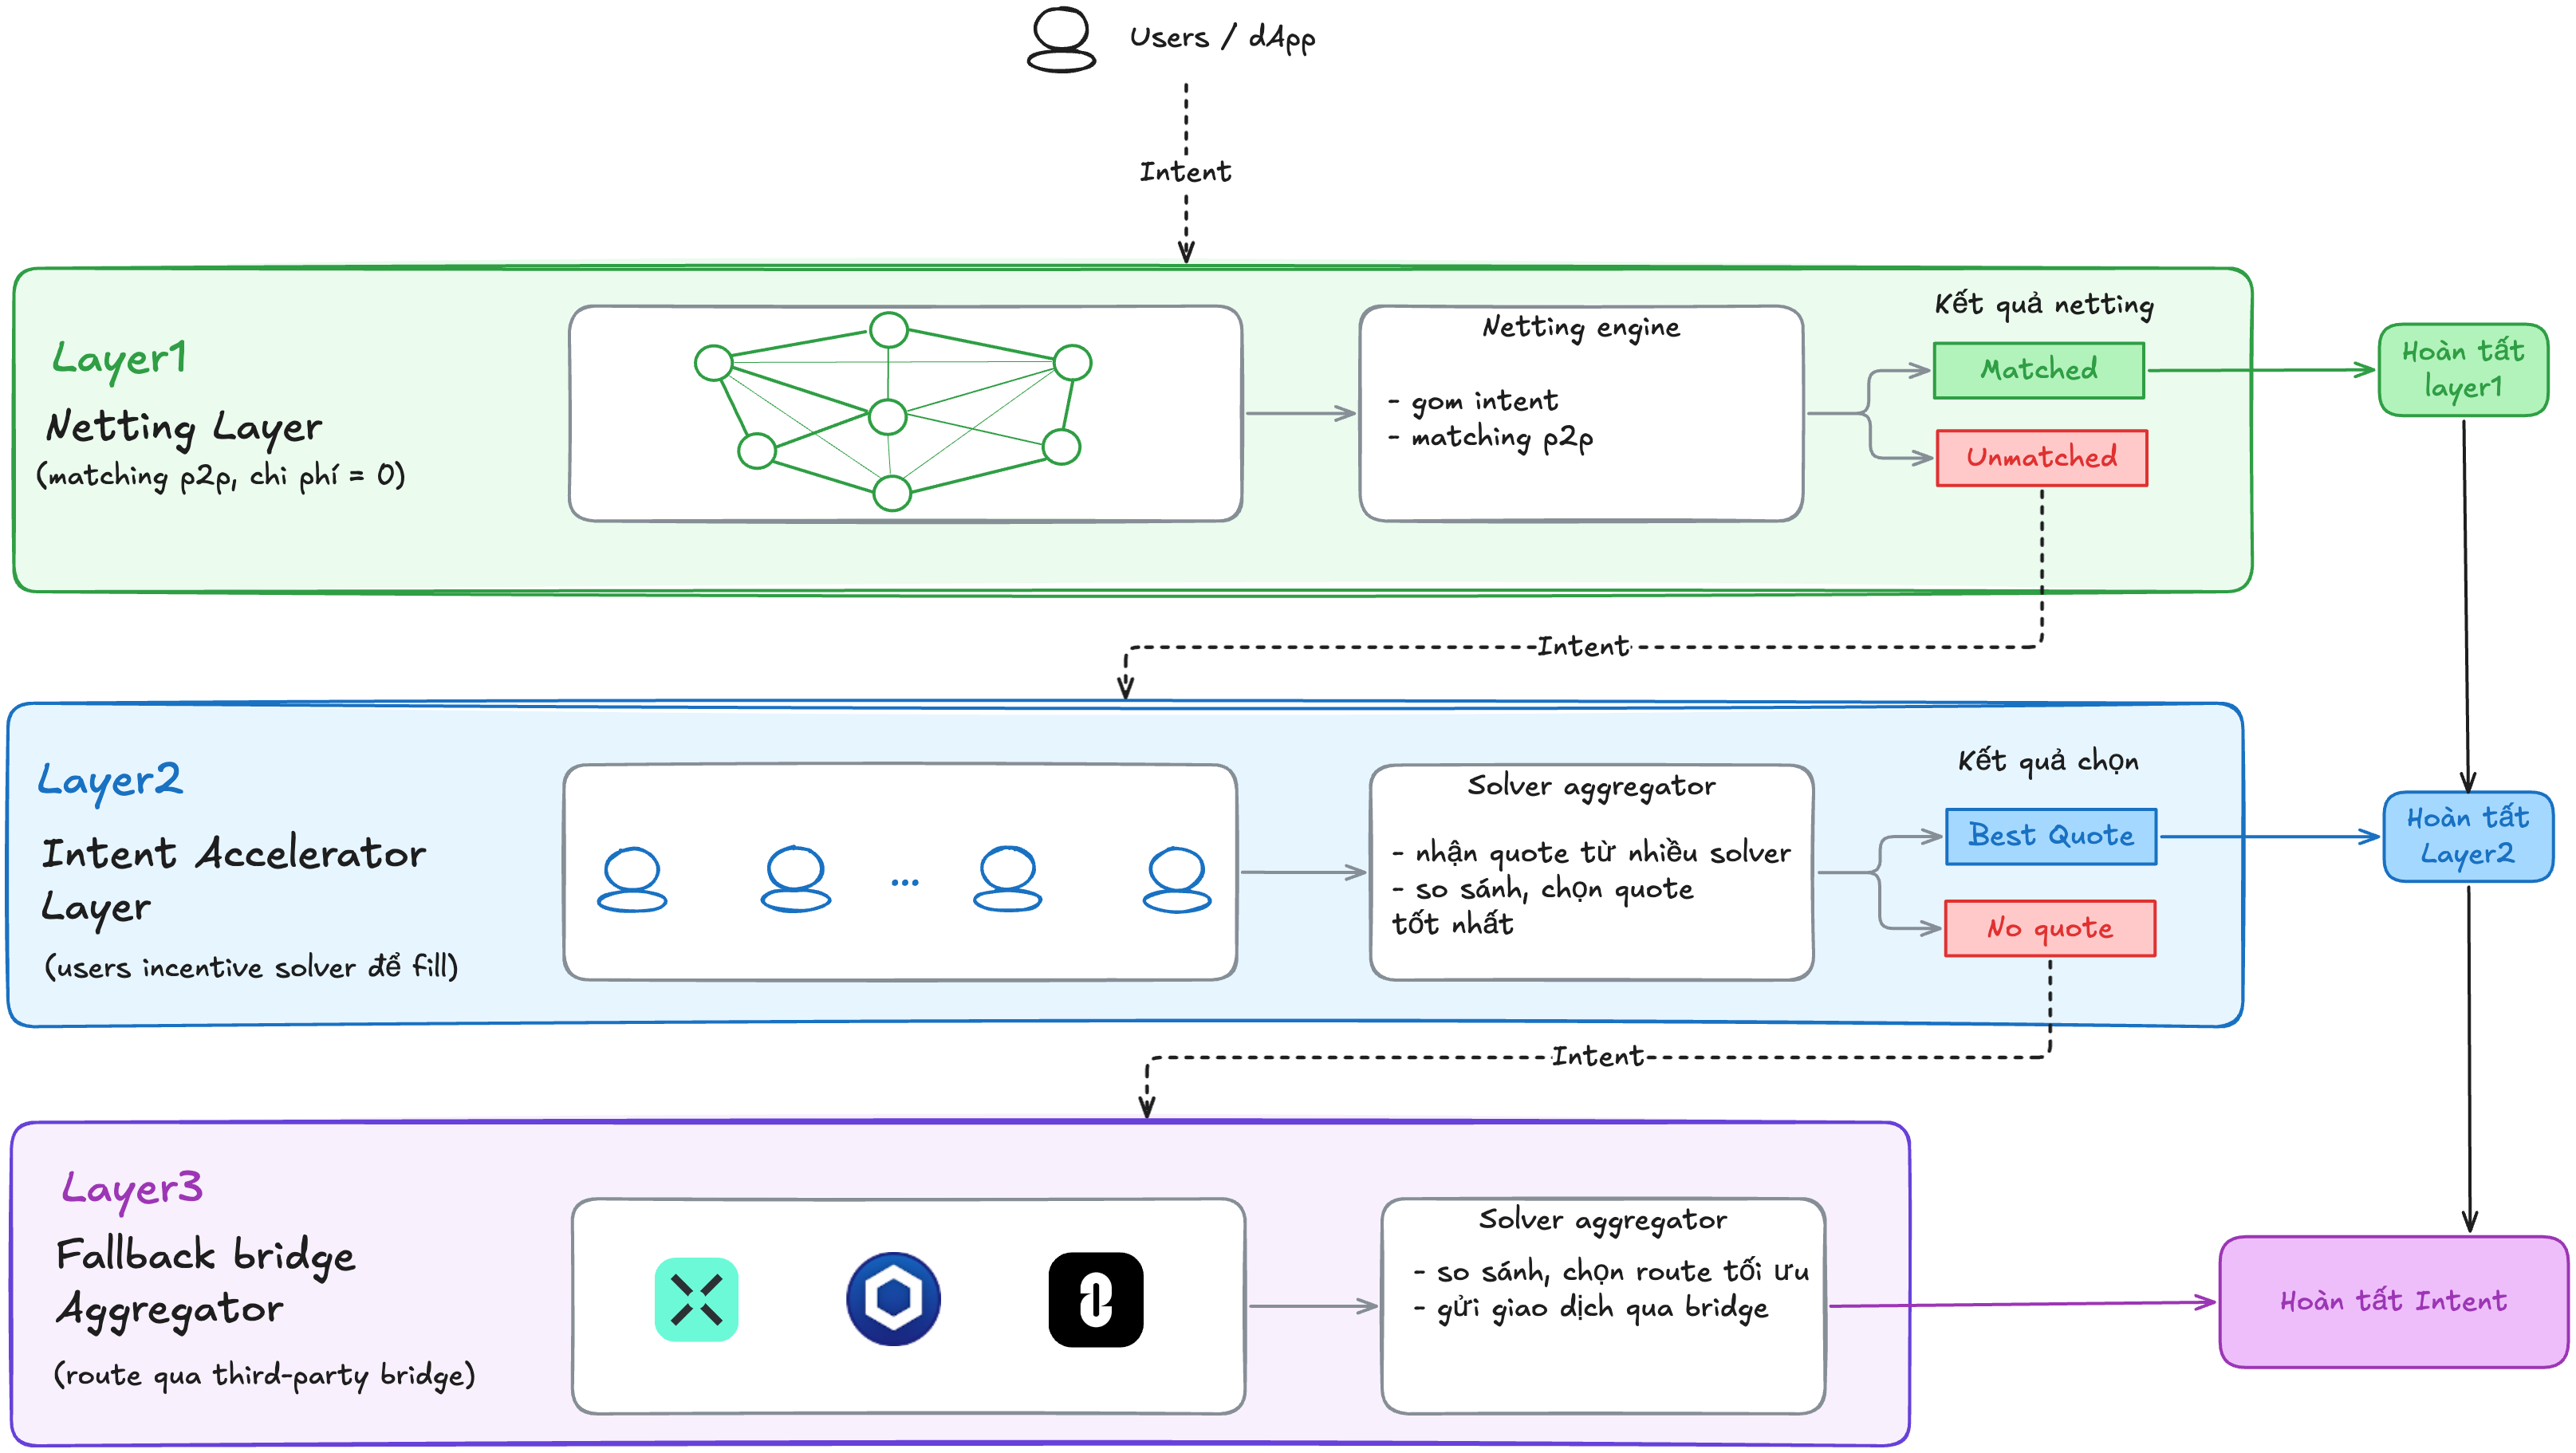
\includegraphics[width=\linewidth]{figures/c3/intent-layer}
  \caption{Vòng đời của một intent qua ba lớp thực thi: bắt đầu ở
  Netting Layer, leo dần xuống Intent Accelerator Layer khi không
  tìm được đối tác bù trừ, và cuối cùng được định tuyến qua
  Fallback Bridge Aggregator nếu cần.}
  \label{fig:intent-lifecycle}
\end{figure}

\paragraph{Ánh xạ các lớp vào thành phần.} Mặc dù ba lớp khác nhau
ở \emph{nguồn thanh khoản} và \emph{cơ chế tìm đối tác}, chúng dùng
chung phần lớn các thành phần đã giới thiệu:

\begin{itemize}
  \item \textbf{Lớp 1} dùng API Gateway, OrderStore, Matching Engine
    (MatchScheduler + MatchingService + Solver), Execution Engine và
    Smart Contract Layer (HTLC).
  \item \textbf{Lớp 2} dùng cùng API Gateway và OrderStore, nhưng
    thay Matching Engine bằng một bộ phát quote tới các solver bên
    ngoài; Execution Engine và HTLC vẫn là kênh thanh toán cuối.
  \item \textbf{Lớp 3} dùng Fallback Bridge Aggregator để chọn và
    gọi adapter bridge phù hợp; bỏ qua HTLC và đi qua kênh thanh
    toán riêng của bridge bên thứ ba.
\end{itemize}

\paragraph{Phạm vi triển khai trong luận văn.}

\begin{itemize}
  \item \textbf{Lớp 1} đã được cài đặt đầy đủ: matching engine, HTLC
    multi-fill, orchestrator. Đây là phần tập
    trung của các tiểu mục thiết kế chi tiết và phần đo benchmark
    trong chương Đánh giá.
  \item \textbf{Lớp 2} được trình bày ở mức thiết kế: interface,
    Dutch auction incentive, lưu đồ tương tác. Cài đặt cụ thể nằm
    ngoài scope.
  \item \textbf{Lớp 3} được trình bày ở mức thiết kế: interface
    \texttt{BridgeAdapter} và danh sách bridge ứng cử
    (\S\ref{sec:fallback-bridge}). Cài đặt cụ thể nằm ngoài scope.
\end{itemize}

Phần Future Work (chương cuối) liệt kê các hạng mục cần hoàn thiện
để Lớp 2 và Lớp 3 đi vào hoạt động đầy đủ.

% =============================================================================
% Draft mục 3.3.7 — Fallback Bridge Aggregator (DESIGN-ONLY)
% =============================================================================

\subsection{Fallback Bridge Aggregator}
\label{sec:fallback-bridge}

\noindent\textbf{Lưu ý phạm vi.} Mục này trình bày
\emph{thiết kế ý đồ} của tầng fallback. Trong scope của luận văn, cài
đặt thực tế chưa được hoàn tất; mã nguồn hiện chỉ chứa interface và
một adapter mẫu. Phần thực thi đầy đủ và đo benchmark được liệt kê
trong Chương Future Work.

\subsubsection*{Lý do tồn tại}

Matching Engine (\S\ref{sec:matching-engine}) chỉ thanh toán được
phần intent có thể tham gia vào một chu trình thoả ngưỡng
$\mathrm{ratio} > x$. Có hai nhóm trường hợp một intent
\emph{không thể} được khớp bởi tầng netting:

\begin{enumerate}
  \item \textbf{Không có đối ứng.} Tại thời điểm intent được đưa
    vào orderbook, không có intent nào trên cặp chuỗi đối ứng có khả
    năng tạo cycle với nó.
  \item \textbf{Cân bằng lệch.} Cycle tồn tại nhưng
    $\mathrm{ratio}$ quá nhỏ — phần khớp được không bù được chi phí
    gas, hoặc phần dư còn lại quá lớn so với nhu cầu của người dùng.
\end{enumerate}

Trong các trường hợp đó, người dùng vẫn cần một con đường để hoàn
tất việc bridge. \emph{Fallback Bridge Aggregator} là tầng cuối
cùng: thay vì cố matching P2P, nó định tuyến intent qua một bridge
"thông thường" — một bridge bên thứ ba đã có thanh khoản thực sự
trên cả hai chuỗi — và chấp nhận trả phí cao hơn để đổi lấy
\emph{tính chắc chắn về thời gian hoàn tất}.

\subsubsection*{Vị trí trong mô hình thực thi ba lớp}

Theo mô hình thực thi ba lớp (\S "Mô hình thực thi ba lớp"), một
intent điển hình đi qua các lớp theo thứ tự ưu tiên:

\begin{enumerate}
  \item \textbf{Netting Layer.} Đợi tối đa $T_{\text{net}}$ giây (mặc
    định: vài tick scheduler). Nếu được matching engine khớp một
    phần hoặc toàn bộ, phần đã khớp đi qua Execution Engine và HTLC.
    Phần dư (nếu có) tiếp tục.
  \item \textbf{Intent Accelerator Layer} (chưa nằm trong scope). Mời
    các solver bên ngoài quote một mức giá riêng cho phần dư;
    người gửi có thể chấp nhận hoặc từ chối. Nếu chấp nhận và solver
    thực hiện, phần dư được thanh toán qua HTLC như một flow đặc
    biệt.
  \item \textbf{Fallback Bridge Aggregator.} Nếu cả hai lớp trên
    không xử lý được trong thời gian $T_{\text{total}}$, phần intent
    còn lại được định tuyến qua một bridge bên thứ ba.
\end{enumerate}

Trật tự này đảm bảo: phần lớn intent hưởng lợi từ phí thấp + thanh
toán P2P (lớp 1), một số ít chấp nhận trade-off (lớp 2), và không
có intent nào bị "treo" vô thời hạn (lớp 3).

\subsubsection*{Các bridge ứng cử viên}

Thiết kế tham khảo ba bridge phổ biến để tích hợp:

\begin{itemize}
  \item \textbf{Across Protocol.} Mô hình intents-based, dùng các
    relayer cạnh tranh. Phù hợp với các cặp Ethereum L1 $\leftrightarrow$ L2 (đặc
    biệt là Arbitrum, Base, Optimism). Phí thường thấp; thời gian
    finalize tính bằng phút.
  \item \textbf{LayerZero.} Generic messaging layer. Tích hợp tốt với
    nhiều chuỗi non-EVM trong tương lai. Mô hình endpoint + DVN
    (Decentralized Verifier Network), tuỳ vào lựa chọn DVN mà chi
    phí và độ trễ khác nhau.
  \item \textbf{Chainlink CCIP.} Cross-Chain Interoperability
    Protocol. Phù hợp khi yêu cầu finality cao và sẵn sàng trả phí
    đáng kể. Mạng đã được tích hợp trên cả ba chuỗi mục tiêu.
\end{itemize}

Tầng aggregator được thiết kế \emph{không khoá vào một bridge cụ
thể}; thay vào đó, nó định nghĩa một interface chung và mỗi bridge
là một adapter implement interface đó.

\subsubsection*{Interface đề xuất}

Theo nguyên tắc đa hình ngầm (structural typing) của TypeScript,
interface tối thiểu của một bridge adapter có dạng:

\begin{verbatim}
interface BridgeAdapter {
  name: string;

  // Lấy quote: phí, ETA, lãi suất bảo đảm
  quote(req: QuoteRequest): Promise<QuoteResponse>;

  // Phát giao dịch bridge; trả về txHash trên chuỗi nguồn
  // và thông tin để theo dõi đến khi hoàn tất trên chuỗi đích
  send(req: SendRequest): Promise<SendResult>;

  // Theo dõi trạng thái của một bridge đang chạy
  status(handle: BridgeHandle): Promise<BridgeStatus>;
}
\end{verbatim}

\texttt{Aggregator} duy trì danh sách các \texttt{BridgeAdapter}, gọi
\texttt{quote} song song, chọn quote tốt nhất theo một hàm chi phí
(thường là $\mathrm{fee} + \mathrm{ETA} \cdot \alpha$ cho hằng số
$\alpha$ phản ánh "giá trị thời gian" của người dùng), rồi gọi
\texttt{send} trên
adapter tương ứng. Trạng thái sau đó được theo dõi và cập nhật vào
\texttt{ExecutionRecord} qua cùng kênh sự kiện như nhánh netting.

\subsubsection*{Câu hỏi mở (đặt cho Future Work)}

\begin{itemize}
  \item \textbf{Tiêu chí kích hoạt fallback.} Hiện thiết kế dựa vào
    timeout đơn lẻ; có thể nâng cấp thành chính sách động dựa trên
    profile rủi ro của người dùng (ví dụ: dùng fallback ngay nếu
    intent có \texttt{deadline} quá gần).
  \item \textbf{Lỗ hổng khi quote.} Quote đáo hạn nhanh; aggregator
    cần xử lý trường hợp quote hết hiệu lực giữa lúc người dùng
    chấp nhận và lúc \texttt{send}. Phương án đề xuất: re-quote và
    yêu cầu re-confirm nếu lệch quá ngưỡng.
  \item \textbf{Tích hợp với accounting nội bộ.} Vì fallback tốn
    phí thực, hệ thống cần ghi rõ phần phí được chuyển cho bridge
    bên thứ ba để đối chiếu báo cáo P\&L. Yêu cầu một bảng phụ
    \texttt{fallback\_executions} trong lược đồ dữ liệu.
\end{itemize}

% =============================================================================
% Draft mục 3.3.8 — Event Bus và Persistence
% =============================================================================

\subsection{Event Bus và Persistence}
\label{sec:event-bus-persistence}

Lớp persistence của hệ thống được thiết kế tách bạch hai mối quan tâm khác nhau. Trạng thái bền (durable state) phải sống sót qua restart tiến trình và là nguồn để rebuild in-memory cache; phần này được cài đặt bằng Postgres. Sự kiện thời gian thực (transient pub/sub) chỉ quan trọng khi đang truyền cho người dùng đang kết nối, không cần lưu trữ; phần này được cài đặt bằng một EventEmitter trong bộ nhớ.

Hai cơ chế này, đặt cạnh nhau, đóng vai trò tương đương với một event log Kafka trong các kiến trúc microservice phổ biến, nhưng với chi phí vận hành thấp hơn nhiều bậc — phù hợp với quy mô MVP và scope của luận văn. Phân tích so sánh được trình bày ở mục Phân tích thiết kế thay thế: Kafka vs Postgres + Emitter trong chương Đánh giá.

\subsubsection{Postgres và lược đồ ba bảng}

Cơ sở dữ liệu được truy cập qua Drizzle ORM (TypeScript-first, không codegen) với connection thuần từ \texttt{postgres-js}. Có ba bảng chính, dưới đây trình bày ngắn gọn (chi tiết cột và index xem \texttt{packages/backend/src/db/schema.ts}).

\subsubsection*{Bảng \texttt{intent\_orders}}

Bảng này có một dòng cho mỗi \texttt{IntentOrder}, với các cột chính gồm \texttt{order\_id} (primary key), \texttt{src\_chain}, \texttt{des\_chain}, \texttt{amount} (\texttt{text}, để giữ độ chính xác bigint), \texttt{incentive\_fee}, \texttt{deadline}, \texttt{created\_at}, \texttt{status} (chuỗi enum \texttt{QUEUED}/\texttt{PARTIAL}/\texttt{MATCHED}/\texttt{EXPIRED}) và \texttt{user\_address}. Bảng phục vụ rebuild orderbook khi \texttt{OrderStore.hydrate()} chạy lúc khởi động.

\subsubsection*{Bảng \texttt{match\_results}}

Đây là bảng append-only ghi mỗi sự kiện match, với các cột chính gồm \texttt{match\_id} (primary key), \texttt{matched\_at}, \texttt{orders} (JSONB --- mảng \texttt{MatchedOrderEntry}), \texttt{cycles} (JSONB) và \texttt{raw\_cycles} (JSONB --- snapshot cạnh từ thuật toán). Việc chọn JSONB cho ba trường mảng là vì hệ thống không bao giờ truy vấn vào trong các trường đó — chỉ ghi và đọc nguyên khối.

\subsubsection*{Bảng \texttt{executions}}

Bảng này lưu trạng thái thực thi mỗi \texttt{matchId}, với các cột \texttt{match\_id} (primary key), \texttt{status} (\texttt{pending}/\texttt{done}/\texttt{error}), \texttt{data} (JSONB) và \texttt{error}. Khác với hai bảng trên, dòng trong bảng này được cập nhật tại chỗ (qua \texttt{INSERT ... ON CONFLICT UPDATE}) khi Orchestrator chuyển trạng thái.

\subsubsection{Lazy initialization của DB client}

Vì module \texttt{db/client.ts} được \texttt{import} sớm (theo cơ chế hoisting của ES Module) trong khi \texttt{dotenv.config()} chỉ chạy sau khi tất cả import hoàn tất, một thiết kế đơn giản đọc \texttt{process.env.DATABASE\_URL} ở top-level sẽ throw lỗi.

Giải pháp được áp dụng là \emph{lazy initialization}. Module export một Proxy đại diện cho Drizzle handle; chỉ khi một thuộc tính của Proxy được truy cập lần đầu, hàm \texttt{getDb()} mới đọc biến môi trường, kết nối Postgres và cache instance lại. Cơ chế này làm cho \texttt{db/client.ts} không phụ thuộc thứ tự import, đồng thời cho phép unit test inject biến môi trường giả lập trước khi truy cập DB lần đầu.

\subsubsection{Mẫu write-through với fail-and-log}

Như đã mô tả ở \S\ref{sec:order-book}, mỗi mutation in-memory được mirror sang Postgres theo kiểu fire-and-forget. Cụ thể, Promise \texttt{insert/update} không được \texttt{await}, và handler \texttt{.catch(err => logDbError(scope, err))} đảm bảo lỗi không trở thành unhandled rejection và được log với namespace cụ thể (\texttt{orders.add}, \texttt{matchResults.add}, \texttt{executions.set}, ...).

Trade-off đã được phân tích ở \S\ref{sec:order-book}: nguy cơ lệch giữa in-memory và DB trong cửa sổ rất ngắn nếu tiến trình crash. Đây là chấp nhận được ở MVP, nhưng phương án thay thế thông qua \emph{outbox pattern} (append event vào một bảng riêng cùng transaction với mutation, sau đó dispatch tách biệt) được kiến nghị trong Future Work.

\subsubsection{\texttt{orderEvents}: in-memory event bus}

Ngoài durable state, hệ thống còn cần một kênh truyền sự kiện lifecycle thời gian thực đến các client đang kết nối qua Server-Sent Events (SSE). \texttt{orderEvents} là một \texttt{EventEmitter} của Node.js, sống trong cùng tiến trình backend và không persist.

Mỗi event là một đối tượng \texttt{OrderEvent} với cấu trúc gồm \texttt{orderId} (định danh order liên quan), \texttt{type} (một trong \texttt{queued | matched | plan | htlc\_created | withdrawn | done | error}), \texttt{message} (thông điệp ngắn cho UI), \texttt{data} (payload có cấu trúc, gồm txHash, chainKey, ...), và \texttt{timestamp} (Unix epoch).

Phía producer, \texttt{OrderStore} phát \texttt{queued} khi một order được \texttt{add()}, và phát \texttt{matched} khi \texttt{addMatchResult()}. \texttt{Orchestrator} phát \texttt{plan}, \texttt{htlc\_created}, \texttt{withdrawn}, \texttt{done}, \texttt{error} trong các bước thực thi của mình. Phía consumer, route \texttt{GET /api/intent/:orderId/events} mở một stream SSE: nó subscribe vào \texttt{orderEvents}, lọc theo \texttt{orderId} truyền vào, và push tuần tự xuống browser. Khi client đóng kết nối, listener được tháo gỡ. Với chỉ một consumer nội bộ (SSE handler), \texttt{EventEmitter} là đủ, không cần Redis pub/sub hay Kafka topic.

% [đã sửa: chuyển các \paragraph{...} và bullet list dạng "tên - mô tả" thành câu liền mạch trong văn xuôi]

